At the end of this worksheet you should be able to  
\begin{itemize}
	\item calculate the speed of waves in air at varying temperatures.
	\item operate the Kelvin temperature scale as an absolute temperature scale.
	\item calculate the intensity of a sound wave at any distance from the source.
	\item calculate the loudness of any sound source including the listener's distance from the source.
	\item apply the principles of standing wave to pipes open on one end or open on both ends.
	\item use the principle of beat frequency to calculate for an unknown frequency.
\end{itemize}


\begin{enumerate}
	\setlength\itemsep{2 in}
	
	\item
	According to the notes, the speed of sound in a gas like air is proportional to the square root of the temperature. But much like when we talked about pressure, we need to use an \emph{absolute} temperature scale. In the SI system the Kelvin temperature scale is an absolute measure of temperature, because \SI{0}{\kelvin} is the lowest conceivable temperature. The relationship of the Kelvin scale to the Celsius scale is that \SI{0}{\kelvin} is \SI{-273.15}{\celsius}. So what is \SI{0}{\celsius} in Kelvin? What is \SI{20}{\celsius} in Kelvin? What is \SI{100}{\celsius} in Kelvin? What is \SI{300}{\kelvin} in Celsius? What is \SI{100}{\kelvin} in Celsius?
	
	\item
	The size of the degrees are the same in both the Kelvin and Celsius temperature scales. So if the air temperature changes from \SI{10}{\celsius} to \SI{36}{\celsius}, by how much does the temperature change in Kelvin? If the air temperature changes by \SI{20}{\celsius}, then how much does the temperature change in Kelvin?
	
	\item
	The Celsius scale has its zero point set at the freezing point of water. While this puts the temperatures that humans most commonly deal with at a useful size, it is not acceptable when using proportionality reasoning. For example, does it make sense to refer to doubling the temperature in the Celsius scale? Is \SI{20}{\celsius} twice the temperature of \SI{10}{\celsius}? If not, what is the proper ratio of these two temperatures? What is the percent change going from \SI{10}{\celsius} to \SI{20}{\celsius}?
	
	\item
	So in these problems in order to find the speed of sound at any temperature, we need to use a known reference speed at a known temperature. We will use the reference speed of sound in air of $v_0 = \SI{331}{m/s}$ at the temperature of $T=\SI{0}{\celsius}$ or $\SI{273.15}{\kelvin}$. So what is the speed of sound at \SI{20}{\celsius}? At what temperature would the speed of sound be \SI{300}{m/s}? At what temperature would it be \SI{400}{m/s}?
	
	\item
	If the temperature of air decreased by 10\%, then by what percent would the speed of sound decrease?
	
	\item
	\SI{40}{\celsius} is just about as hot as it ever gets in Alabama in the summer and \SI{-15}{\celsius} is just about as cold as it ever gets in the winter. What is this ratio of temperatures and what is the ratio of speeds of sound in the hottest day of the summer to speeds of sound in the coldest night in the winter? What is the speed of sound at these temperatures?
	
	\item  
	A firework explodes releasing \SI{100}{\kilo\joule} of energy in \SI{0.001}{\second}. What power is this? If 10\% of this power goes into sound energy what power is that? What is the intensity of this sound \SI{1}{\meter} away from the explosion? What is the intensity \SI{10}{\meter} away? \SI{100}{\meter} away?
	
	\item
	If the intensity of music from a loudspeaker at a concert is \SI{1}{\watt/\meter^2} at a distance of \SI{1}{m} away, then what is the intensity \SI{10}{\meter} away? \SI{100}{\meter} away? 
	
	\item
	For all of the intensities in the previous problems, calculate their sound level (i.e loudness) relative to the threshold of hearing, $I_0=\SI{e-12}{\watt/\meter^2}$.
	
	\item
	If the sound level at the location of your ear is \SI{60}{\decibel}, what is the intensity of sound? If your eardrum (also apparently called the tympanic membrane)has a diameter of \SI{0.5}{cm}, then what power is delivered to your eardrum?
	
	\item
	The intensity of a sound is doubled. What is the difference in the sound level \emph{change}? {Hint: subtract the sound level of $2I$ and $I$ and then use the properties of logarithms that $\log A - \log B = \log\left(A/B\right)$}
	
	\item 
	The smallest change in sound level that humans can detect is about \SI{1}{\decibel}. What is the ratio of intensity does this represent?
	\bigskip
	\item
	What is the sound level \SI{1}{\meter} away from a \SI{100}{\watt} sound source? What is it \SI{2}{\meter} away? Plot this change in sound level as a function of distance away from the source. If you double your distance away from a source of sound how much does the sound level change?\bigskip
	
	\item
	What is the fundamental frequency and wavelength of a \SI{1}{m} long pipe open at both ends at \SI{24}{\celsius}? What is the fundamental frequency and wavelength of the same pipe if it is closed at one end? For each pipe, what is the next highest frequency that supports a standing wave in the pipe?
	
	\item 
	On a guitar each string has a different mass density and tension, but also the fret board of the guitar allows you to shorten the length of each string. The frequency of the top E string at is full length of about a meter is about 164 Hz. 
	\begin{itemize}
		\setlength\itemsep{2 in}
		\item If I press the string on a fret to half the length of the string, then how much does the fundamental frequency change? State it as a difference, and a ratio, and a percent change.
		\item On a guitar, the frets are spaced so that there are 12 divisions. So if the divisions are equally spaced (they aren't for reasons that are outside the scope of this problem) then how much does the length change with each fret?
		\item So how much does each fret shorten the string by? If I press on the first fret by how much did the frequency change? As a difference and a percent change?
		\item What about the next fret as a difference and percent change?
	\end{itemize}
	
	\item
	The speed of a wave on a \SI{1}{\meter} long string is \SI{100}{m/s}. What is the fundamental wavelength and frequency? If this string is in air at \SI{25}{\celsius} what is the frequency and wavelength of the pressure wave? If the temperature drops to \SI{10}{\celsius}, by how much does the fundamental frequency change?
	
	\item
	What are the three lowest standing wave frequencies of a \SI{2}{m} long pipe that is open on both ends when the speed of sound is \SI{340}{m/s}? What if the pipe were closed on one end?
	
	\item
	Two strings of a guitar are being played at the same time. One string has a frequency of 400Hz. A beat frequency of 5 Hz can be heard. What are the possibilities for the frequency of the second string? If the tension in the second string is increased, and the beat frequency decreases to 2Hz, then what can you conclude about the frequency of the second string before it was tightened? By what percent was the tension in the string increased? By what percent would the tension need to be increased in order to eliminate the beating?
	
	\item
	Imagine the last problem if tightening the string had \emph{increased} the beat frequency. What would you conclude about the original frequency then?
	
	\newpage
	\centering
	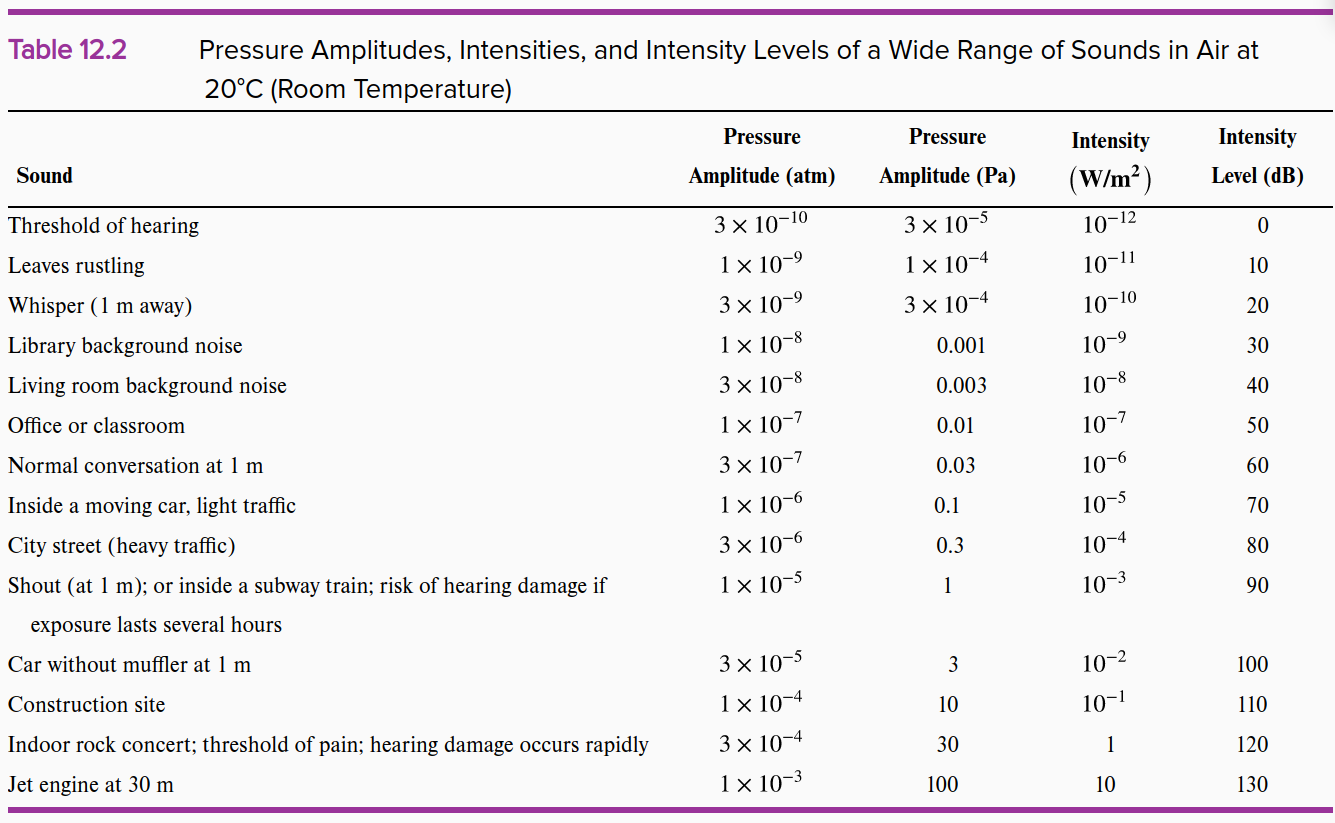
\includegraphics[width=\linewidth]{week14-table-sound-level}
	
	
\end{enumerate}